\documentclass[a4paper]{jpconf}
\usepackage{graphicx}

\usepackage{tikz}
\usepackage{bm}
\usepackage{amsmath}

\graphicspath{{pictures/}}


\begin{document}
\title{Modelling dynamic processes in a nuclear reactor by state change modal method}

\author{A V Avvakumov$^1$, V F Strizhov$^2$, P N Vabishchevich$^{2,3}$ and A O Vasilev$^3$}

\address{$^1$ National Research Center Kurchatov Institute, Moscow, Russia}
\address{$^2$ Nuclear Safety Institute of RAS, Moscow, Russia}
\address{$^3$ North-Eastern Federal University, Yakutsk, Russia}

\ead{haska87@gmail.com}

\begin{abstract}
Modelling of dynamic processes in nuclear reactors is carried out, mainly, on
the basis of the multigroup diffusion approximation for the neutron flux. 
The basic model includes a multidimensional set of coupled parabolic equations and
ordinary differential equations.
Dynamic processes are modelled by a successive
change of the reactor states, which are characterized by given coefficients of the equations. 
It is considered that the transition from one state to another occurs instantaneously.
In the modal method the approximate solution is represented as eigenfunction expansion. 
The numerical-analytical method is based on the use of dominant time-eigenvalues of
a multigroup diffusion model taking into account delayed neutrons. 
%For each reactor state the eigenvalues and eigenfunctions of the $\alpha$-eigenvalue problem are calculated in advance.
%This provides very fast calculations in real-time scale.
%Numerical simulations of the dynamic process were performed in the framework of the
%two-group approximation for the VVER-1000 reactor test model. 
%The last is characterized by the fact that some eigenvalues are complex.
%The dynamic model includes two reactor states, namely the regular regime of the supercritical state with further transition to the subcritical state.
%The results of the dynamic process simulation demonstrate the acceptable accuracy in calculation of neutron power and delayed neutrons source in comparison with the direct dynamic calculation.
\end{abstract}

\section{Introduction}
These guidelines show how to prepare articles for publication in \jpcs\ using \LaTeX\ so they can be published quickly and accurately. Articles will be refereed by the \corg s but the accepted PDF will be published with no editing, proofreading or changes to layout. It is, therefore, the author's responsibility to ensure that the content and layout are correct.  This document has been prepared using \cls\ so serves as a sample document. The class file and accompanying documentation are available from \verb"http://jpcs.iop.org".
These guidelines show how to prepare articles for publication in \jpcs\ using \LaTeX\ so they can be published quickly and accurately. Articles will be refereed by the \corg s but the accepted PDF will be published with no editing, proofreading or changes to layout. It is, therefore, the author's responsibility to ensure that the content and layout are correct.  This document has been prepared using \cls\ so serves as a sample document. The class file and accompanying documentation are available from \verb"http://jpcs.iop.org".
These guidelines show how to prepare articles for publication in \jpcs\ using \LaTeX\ so they can be published quickly and accurately. Articles will be refereed by the \corg s but the accepted PDF will be published with no editing, proofreading or changes to layout. It is, therefore, the author's responsibility to ensure that the content and layout are correct.  This document has been prepared using \cls\ so serves as a sample document. The class file and accompanying documentation are available from \verb"http://jpcs.iop.org".

\section{Problem statement}
The neutron flux is modelled in multigroup diffusion approximation. The neutron dynamics is considered in the bounded convex two-dimensional or three-dimensional area  $\Omega$ ($\bm x = \{x_1, ..., x_d\} \in \Omega, \ d = 2,3$) with boundary $\partial \Omega$. The neutron diffusion is described by:
\begin{equation}\label{1}
\begin{split}
V(t) \frac{d \bm \phi}{d t} + (D(t)+S(t)) \bm \phi &= R(t) \bm \phi + B(t)\bm c,
\\
\frac{d \bm c}{d t} + \Lambda(t)\bm c &= Q(t) \bm \phi. 
\end{split}
\end{equation}  
Where vectors $\bm \phi = \{\phi_1, \phi_2, ..., \phi_G\}$, $\bm c = \{c_1, c_2, ..., c_M\}$ 
and matrices:
\[
\begin{aligned}
 V = (v_{g g'}), \quad v_{g g'} = \delta_{g g'} v_g^{-1}, \quad 
 D = (d_{g g'}), \quad d_{g g'} = - \delta_{g g'} \nabla \cdot D_g \nabla, \\
 S = (s_{g g'}), \quad  s_{g g'} =  \delta_{g g'} \Sigma_g - \Sigma_{s,g'\rightarrow g}, \quad R  = (r_{g g'}), \quad  r_{g g'} = (1-\beta)\chi_g \nu \Sigma_{fg'}, \\
 B = (b_{g m}), \quad b_{g m}  = \widetilde{\chi}_g \lambda_m, \quad
\Lambda = (\lambda_{m m'}), \quad  \lambda_{m m'} = \lambda_m \delta_{m m'}, \\
 Q = (q_{mg}), \quad  q_{mg}  = \beta_m \nu \Sigma_{fg}, \quad g, g' = 1,2, ..., G, \quad 
 m, m' = 1,2, ....,M,
\end{aligned}
\]
where
$\delta_{g g'}$ is the Kronecker symbol. We shall use the set of vectors $\bm \phi$, whose components 
satisfy the albedo boundary conditions: 
\begin{equation}\label{2}
 D_g\frac{\partial \phi_g}{\partial n} + \gamma_g \phi_g = 0, \quad 
 \quad g = 1,2, ..., G ,
\end{equation}
where $n$ --- outer normal to the boundary $\partial \Omega$.

Here $\phi_g(\bm x,t)$ --- neutron flux of $g$ group at point $\bm x$ and time $t$,
$G$ --- number of energy groups,
$v_g$ --- effective velocity of neutrons in the group $g$,
$D_g(\bm x)$ --- diffusion coefficient, $\Sigma_{rg}(\bm x,t)$ --- removal cross-section,
$\Sigma_{s,g'\rightarrow g}(\bm x,t)$ --- scattering cross-section from group $g'$ to group $g$,
$\beta$ --- effective fraction of delayed neutrons, $\chi_g$, $\widetilde{\chi}_g$  --- spectra of prompt and delayed neutrons, 
$\nu\Sigma_{fg}(\bm x,t)$ --- generation cross-section of group $g$,
$c_m$ --- density of sources of delayed neutrons of $m$-type,  $\lambda_m$ --- decay constant of sources of delayed neutrons,
$M$ --- number of types of delayed neutrons,  and $\beta_m$ is a fraction of delayed neutrons of $m$-type:
\[
 \beta = \sum_{m=1}^{M} \beta_m .
\] 

The Cauchy problem is formulated for equations (\ref{1})  when 
\begin{equation}\label{3}
 \bm \phi(0) = \bm \phi^0,
 \quad   \bm c(0) = \bm c^0,
\end{equation} 
where taken into account $\bm \phi^0 = \{ \phi_1^0,  \phi_2^0, ...,  \phi_G^0 \}$,  $\bm c^0 = \{c_1^0, c_2^0, ..., c_M^0\}$.

\section{State change modal method}
The nuclear reactor is always non-stationary. The limiting case of reaching a steady state (critical reactor) is observed only for certain coefficients of the equations system (\ref{1}). We will use the following simplified description of the dynamic processes in a nuclear reactor.

In selected time interval, the non-stationary neutron flux is determined by the nuclear reactor state. The state of the reactor is characterized by the constant coefficients of the system of multigroup diffusion equations (\ref{1}). Dynamic processes in a nuclear reactor can be considered as a change of states  (see  Fig.\ref{fig:1}). 
At a certain time $t = t_s, \ s = 1,2, ...$ an instantaneous change of state occurs. The state $s$ is defined by the parameters in equations  (\ref{1}):
\[
 V(t) = V(t_s), \quad  D(t) = D(t_s), \quad  S(t) = S(t_s), \quad  R(t) = R(t_s), \quad  B(t) = B(t_s),
\] 
\[
 \Lambda(t) = \Lambda(t_s), \quad  Q(t) = Q(t_s),
 \quad t_{s-1} < t \leq t_s, \quad s = 1,2, ... 
\] 


Simulation of the dynamic behavior of the reactor consists in solving the sequence of subtasks for the individual states of the reactor. The initial condition for the state $s$ (at $t = t_{s-1}$) is the final state of the reactor for the state $s-1$.

\begin{figure}[h] 
  \begin{center}
\vspace{5mm} 
    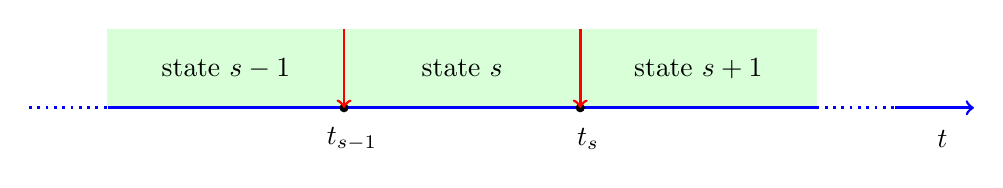
\begin{tikzpicture}
      \filldraw [color=green!15] (0,0) rectangle +(9,1);
      \draw [dotted, line width=1, color=blue] (-1,0) -- (0,0);
      \draw [line width=1, color=blue] (0,0) -- (9,0);
      \draw [dotted, line width=1, color=blue] (9,0) -- (10,0);
      \draw [->, line width=1, color=blue] (10,0) -- (11,0);
      \filldraw [black] (3,0) circle (0.05);
      \filldraw [black] (6,0) circle (0.05);
      \draw  (1.5,0.5) node {state $s-1$};  
      \draw  (4.5,0.5) node {state $s$};  
      \draw  (7.5,0.5) node {state $s+1$};  
      \draw  (3.1,-0.4) node {$t_{s-1}$}; 
      \draw  (6.1,-0.4) node {$t_{s}$}; 
      \draw  (10.6,-0.4) node {$t$}; 
      \draw [->, line width=1, color=red] (3,1) -- (3,0);
      \draw [->, line width=1, color=red] (6,1) -- (6,0);
    \end{tikzpicture}
    \caption{State change scheme.} 
   \label{fig:1}
  \end{center}
\end{figure}

An approximate description of the non-stationary process at a separate stage is based on modal approximation. An approximate solution is sought in the form of decomposition in eigenfunctions of time and $\alpha$-eigenvalue problem. Finite-element approximation in space is used.

Let's $\bm u = \{\bm \phi, \bm c\}$. Rewrite the system of equations (\ref{1}) as
\begin{equation}\label{4}
 \bm B \frac{d \bm u}{d t} + \bm A \bm u = 0,
 \quad t_{s-1} < t \leq t_s,
\end{equation} 
with constants
\[
 \bm A = 
 \begin{pmatrix}
 D(t_s)+S(t_s) - R(t_s) &  - B(t_s) \\
 - Q(t_s) & \Lambda(t_s) 
 \end{pmatrix} ,
 \quad  \bm B = 
 \begin{pmatrix}
 V(t_s) & 0 \\
 0 & I 
 \end{pmatrix} ,
\] 
where $I$ is the identity matrix. Initial conditions:
\begin{equation}\label{5}
 \bm u(t_{s-1}) = \bm u^s .
\end{equation} 

After approximating over the space by the finite element method from (\ref{4}), (\ref{5}) 
we turn to the Cauchy problem for a linear system of ordinary differential equations with constant coefficients:
\begin{equation}\label{6}
 \bm B_h \frac{d \bm u_h}{d t} + \bm A_h \bm u_h = 0,
 \quad t_{s-1} < t \leq t_s,
\end{equation}   
\begin{equation}\label{7}
 \bm u_h(t_{s-1}) = \bm u_h^s ,
\end{equation} 
where $h$ is the discretization parameter. The main feature of the problems we are considering is that the matrices $\bm A_h$ and $\bm B_h$ 
are real and asymmetric.

The modal approximation corresponds to the representation of the approximate solution  ($\bm u_h \approx \bm u_N$) of problem   (\ref{6}), (\ref{7}) in the following form
\begin{equation}\label{8}
 \bm u_N(\bm x, t) =
 \sum_{n=1}^{N} a_n(t) \bm w_n(\bm x),
\end{equation} 
where $N$ is the number of dominant eigenvalues of the spectral problem, 
$\bm w_n(\bm x)$ --- corresponding eigenfunctions.

Let us define eigenfunctions and eigenvalues as the solution of the  $\alpha$-eigenvalue problem:
\begin{equation}\label{9}
 \bm A_h \bm v = \lambda  \bm B_h \bm v .
\end{equation} 

In the general case, eigenfunctions and eigenvalues of the spectral problem  (\ref{9}) are complex.
Taking into account the validity of the matrix coefficients  $\bm A_h, \ \bm B_h$ complex eigenvalues appear as pairs of complex conjugate numbers. For example, we have a pair of $n,n+1$: 
\[
 \lambda_{n+1} = \mathrm{Re} \lambda_n - i \mathrm{Im} \lambda_n . 
\] 
Then in the representation  (\ref{8}) we obtain
\[
\begin{split}
 a_n(t) \bm w_n(\bm x) & = b_n \mathrm{Re} \big ( \exp(-\lambda_n (t-t_{s-1})) \bm v_n(\bm x) \big ), \\
 a_{n+1}(t) \bm w_{n+1}(\bm x) & = b_{n+1} \mathrm{Im} \big ( \exp(-\lambda_n (t-t_{s-1})) \bm v_n(\bm x) \big ) .
\end{split}
\] 

A special attention should be paid to define the coefficients $a_n(t_{s-1}) = b_n, \ n = 1,2, ..., N$.
For this, the initial condition (\ref{7}) is involved. For example, in the case of real eigenvalues, we have
\[
 \bm u_h^s (\bm x) = \sum_{n=1}^{N_h} b_n \bm v_n(\bm x) .
\] 
This representation is not very suitable for practical use with modal approximation, when we work only with dominant eigenfunctions.  

The initial condition includes two components  $\bm u_h^s (\bm x) = (\bm \phi_h^s (\bm x), \bm c_h^s (\bm x))$.
Dynamic behaviour of these components is due to different time-scale processes. Delayed neutrons source determines slow processes, when  $\bm c(\bm x,t)$ changes slightly with the reactor state change. In contrast, neutron flux $\bm \phi(\bm x,t)$ determines fast processes when the reactor state changes. By virtue of this separation of dynamic processes, we model the slow phase of the dynamics of the reactor with modal approximation and orientate ourselves on the approximate prediction of the initial state for delayed neutrons, only the function  $\bm c_h^s (\bm x)$ is approximated. The approximation  $\bm \phi_h^s (\bm x)$ is not of interest to us; we do not model a fast phase of the state change.

The standard approach for the decomposition of the function  $\bm u_h^s (\bm x) $ 
over the system of non-orthogonal functions $\bm v_n(\bm x), \ n = 1,2, ..., N_h$ 
consists in using the biorthogonal system of functions 
\cite{henry1975nuclear,brezinski1991biorthogonality}. 
Consider the spectral problem adjoint to (\ref{9})  
\begin{equation}\label{10}
 \bm A_h^T \widetilde{\bm v}  = \lambda  \bm B_h^T \widetilde{\bm v} .
\end{equation} 
The eigenfunctions of problems  (\ref{9}) and (\ref{10}) are orthogonal \cite{Laub2005,Ortega1987}  in the sense of the equality
\[
  (\bm B_h \bm v_n, \widetilde{\bm v}_m)= 0, 
  \quad m \neq n,
  \quad m, n = 1,2, ..., N_h , 
\] 
where $(\cdot, \cdot)$ means corresponding scalar product. 
In view of this, one can obtain
\begin{equation}\label{11}
 b_n = \frac{1}{(\bm B_h \bm v_n, \widetilde{\bm v}_n)} (\bm u_h^s, \bm B_h \widetilde{\bm v}_n),
 \quad n = 1,2, ..., N_h .  
\end{equation} 
With known solutions of the spectral problems  (\ref{9}), (\ref{10}) the solution is represented in the form (\ref{8}), (\ref{11}).

In the approximate solution of problem   (\ref{6}), (\ref{7}) only the first $N$ coefficients  $b_n$ in (\ref{11}) are used (see (\ref{8})):
\begin{equation}\label{12}
 \bm c_h^s (\bm x) \approx  \sum_{n=1}^{N} b_n \bm c_n(\bm x) ,
\end{equation} 
where $\bm v_n (\bm x) = (\bm \phi_n (\bm x), \bm c_n (\bm x))$.
In this case, the spectral problems  (\ref{9}), (\ref{10}) are solved for $N$ dominant 
eigenvalues.
The solution of the adjoint spectral problem is involved only for calculating the initial condition coefficients. 
%This complication of the problem is not always justified. Therefore, it is worth to use simpler algorithms for obtaining the coefficients  $b_n, \ n = 1,2, ..., N$ in (\ref{12}).
%We can define them, for example, based on linear least squares  \cite{LSPk1996,verdu2014modal}.
%In this case, one can obtain
%\begin{equation}\label{13}
% (\bm r_N, \bm r_N) \longrightarrow \min, 
% \quad \bm r_N (\bm x)  = \bm c_h^s (\bm x) -  \sum_{n=1}^{N} b_n \bm c_n(\bm x) .
%\end{equation} 
%To find the coefficients, a system of linear equations is solved. 

The most favourable case -- when we use single delayed neutron group ---
M = 1 (see \ref{2}). In common case we have to rely on the second level to distinguish
fast and slow processes. Delayed neutrons groups differ in their characteristic
times, which depnd on constants $\lambda_m, m = 1, 2, ..., M$ (see \ref{2}). At asymptotic
stage the relatively slow processes prevail. It is due to the longest-lived delayed
neutron precursor --- the smallest $\lambda_m, m = 1, 2, ..., M$. Other groups are not
taken into account using the modal approach.

The state change modal method is based on the following calculating scheme.
\begin{description}
 \item[Off-line calculation.] Calculation of the coefficients of the mathematical model of the multigroup diffusion approximation for the isolated reactor states, which is performed in advance. The status passport also includes calculated dominant eigenvalues and eigenfunctions of the  $\alpha$-eigenvalue problem (\ref{9}). 
These data can be supplemented by dominant eigenvalues and eigenvalues of the conjugate eigenvalue problem (\ref{10}).
 \item[On-line calculation.] Real-time modeling is carried out on the basis of the modal solution of the problem  (\ref{6}), (\ref{7}).
The coefficients in the representation  (\ref{12}) are calculated from the initial condition using (\ref{11}). The solution for other time intervals is determined according to (\ref{8}).
\end{description}  

\section{The test: the dynamics of the VVER-1000 reactor during the transition from the supercritical mode to the subcritical mode} 

A test problem for a VVER-1000 reactor without a reflector  \cite{chao} 
is considered in the two-dimensional approximation ($\Omega$ is a reactor core cross-section). A two-group approximation is used taken into account delayed neutrons. 

\subsection{General description} 

The geometric model of the VVER-1000 core consists of a set of hexagonal-shaped cassettes and is shown in Fig.\ref{fig:2}, where fuel assemblies of various types are shown. The assembly ''wrench''  size is 23.6 cm.

\begin{figure}[h]
  \begin{center}
    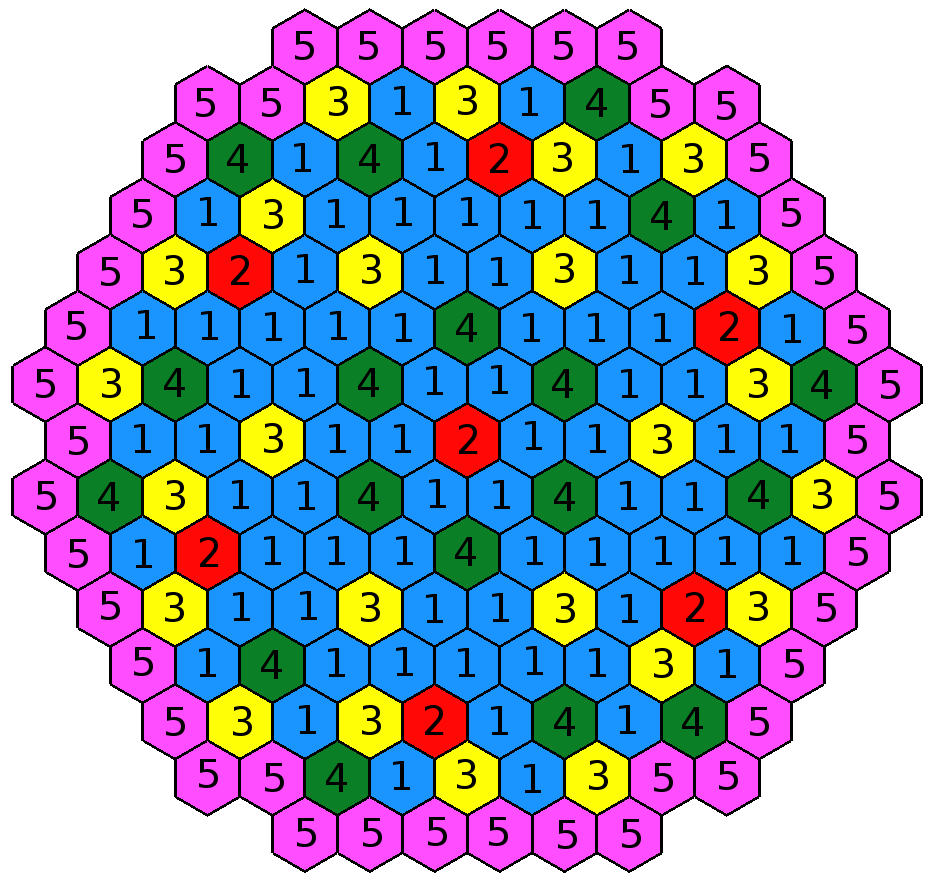
\includegraphics[width=0.5\linewidth] {2.png}
	\caption{Geometrcial model of the VVER-1000 reactor core.}
	\label{fig:2}
  \end{center}
\end{figure} 

For an approximate solution of the problem, regular triangular grids are used. The number of triangles per cassette $\kappa$  varies from 6 to 96. %(Fig.\ref{fig:3}). 

%\begin{figure}[h]
%  \begin{center}
%\begin{minipage}{0.15\linewidth}
%\center{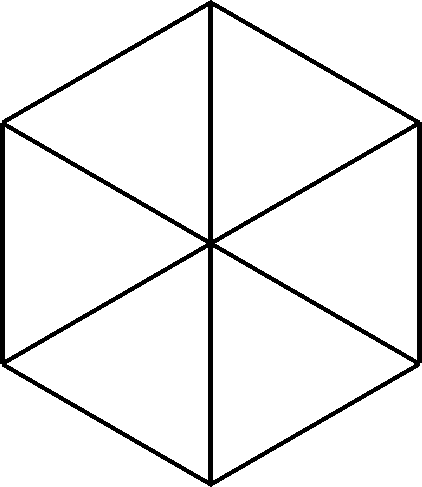
\includegraphics[width=1\linewidth]{3-1.png}}\\
%\end{minipage}
%\hspace{20pt}
%\begin{minipage}{0.15\linewidth}
%\center{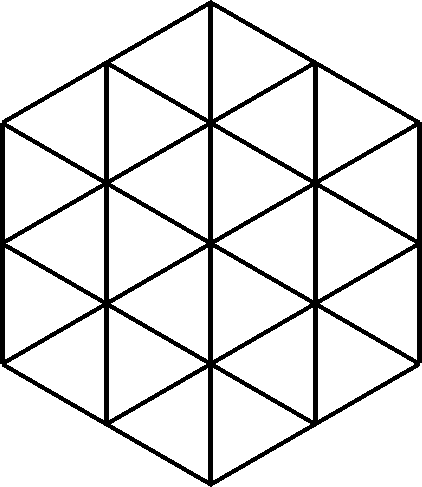
\includegraphics[width=1\linewidth]{3-2.png}}\\
%\end{minipage}
%\hspace{20pt}
%\begin{minipage}{0.15\linewidth}
%\center{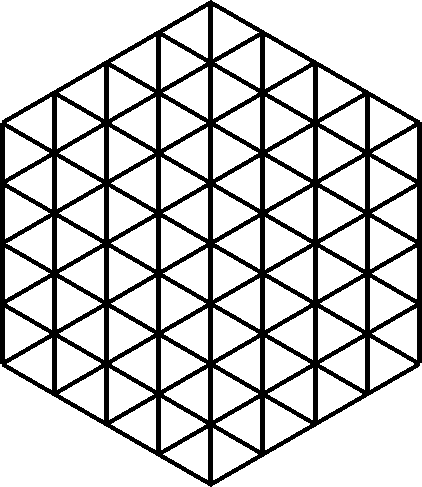
\includegraphics[width=1\linewidth]{3-3.png}}\\
%\end{minipage}
%\caption{Discretization of assembly into 6, 24 and 96 finite elements.}
%\label{fig:3}
%  \end{center}
%\end{figure}

\begin{table}[h]
\caption{Diffusion neutronics constants for VVER-1000}
\label{t-1}
\begin{center}
\begin{tabular}{cccccc}
\br
Material & 1 & 2 & 3 & 4 & 5\\
\mr
$D_1$ & 1.38320e-0 & 1.38299e-0  & 1.39522e-0  & 1.39446e-0  & 1.39506e-0 \\
$D_2$ & 3.86277e-1 & 3.89403e-1 & 3.86225e-1 & 3.87723e-1 & 3.84492e-1 \\
$\Sigma_1 + \Sigma_{s,1\rightarrow 2}$ & 2.48836e-2 & 2.62865e-2 & 2.45662e-2 & 2.60117e-2 & 2.46141e-2\\
$\Sigma_2$ & 6.73049e-2 & 8.10328e-2 & 8.44801e-1 & 9.89671e-2 & 8.93878e-2\\
$\Sigma_{s,1\rightarrow 2}$ & 1.64977e-2 & 1.47315e-2 & 1.56219e-2 & 1.40185e-2 & 1.54981e-2\\
$\nu\Sigma_{f1}$ & 4.81619e-3 & 4.66953e-3 & 6.04889e-3 & 5.91507e-3 & 6.40256e-3\\
$\nu\Sigma_{f2}$ & 8.46154e-2 & 8.52264e-2 & 1.19428e-1 & 1.20497e-1 & 1.29281e-1\\
\br
\end{tabular}
\end{center}
\end{table}

The supercritical state of the reactor is characterized by a set of coefficients, which are given in Table \ref{t-1}. 
The following boundary conditions (\ref{3}) are used:  $\gamma_g = 0.5, \ g = 1,2$.  
The following delayed neutrons parameters are used: one group of delayed neutrons with effective fraction $\beta_1 = 6.5\cdot10^{-3}$ and decay constant $\lambda_1 = 0.08$ s$^{-1}$. 
Neutron velocity  $v_1 = 1.25 \cdot 10^7$ cm/s and $v_2 = 2.5 \cdot 10^5$ cm/s.

\subsection{Supercritical state: $\alpha$-eigenvalue problem} 

Below the results of a numerical solution of the $\alpha$-eigenvalue problem (\ref{9}) are presented. 
%In the framework of the two-group approximation and taking into account the delayed neutrons, one can write 
%\begin{equation}\label{23}
%\begin{split}
% - \nabla \cdot D_1 \nabla \varphi_1  + \Sigma_1 \varphi_1 + \Sigma_{s,1\rightarrow 2} \varphi_1  & \\
% - (1 - \beta_1)(\nu \Sigma_{f1} \varphi_1 + \nu \Sigma_{f2} \varphi_2) - \lambda_1 s & = \lambda^{(\alpha)} \frac{1}{v_1}   \varphi_1, \\
% - \nabla \cdot D_2 \nabla \varphi_2  + \Sigma_2 \varphi_2  - \Sigma_{s,1\rightarrow 2} \varphi_1  
% & = \lambda^{(\alpha)} \frac{1}{v_2}   \varphi_2,\\
% \lambda_1 s - \beta_1(\nu \Sigma_{f1} \varphi_1 + \nu \Sigma_{f2} \varphi_2) & = \lambda^{(\alpha)} s. 
%\end{split}
%\end{equation} 
The dominant eigenvalues $\alpha_n = \lambda_n^{(\alpha)}, \ n = 1,2, ..., N$ are searched for at
\[
 \mathrm{Re}  \lambda_1^{(\alpha)} \leq  \mathrm{Re}  \lambda_2^{(\alpha)} \leq ... 
 \leq \mathrm{Re}  \lambda_N^{(\alpha)} \leq ...\, \leq \mathrm{Re}  \lambda_{N_h}^{(\alpha)}.
\]
Similar calculations of the eigenvalues for the VVER-1000 test problem without delayed neutrons can be found in \cite{avvakumov2017spectral}. 

\begin{table}[h]
\caption{Eigenvalues $\alpha_n = \lambda_n^{(\alpha )}, \ n = 1,2, ..., 5$}
\label{t-2}
\begin{center}
\begin{tabular}{cccccc}
\br
$p$ & $\kappa$ & $\alpha_1$ &  $\alpha_2, \alpha_3$ &  $\alpha_4, \alpha_5$ \\ 
\mr
& 6 & -0.22557  & 0.04241 $\mp$ 3.08808e-06$i$  & 0.06588 $\mp$ 4.80449e-07$i$  \\
1 & 24 & -0.82690  & 0.03777 $\mp$ 5.37884e-06$i$  & 0.06489 $\mp$ 1.37315e-06$i$ \\
& 96 & -1.74998  & 0.03619 $\mp$ 5.69002e-06$i$  & 0.06456 $\mp$ 1.40299e-06$i$ \\
\mr
& 6 & -2.10154  & 0.03592 $\mp$ 4.96474e-06$i$  & 0.06452 $\mp$ 1.21320e-06$i$ \\
2 & 24 & -2.46601  & 0.03562 $\mp$ 5.78277e-06$i$  & 0.06445 $\mp$ 1.40897e-06$i$ \\
& 96 & -2.50375  & 0.03559 $\mp$ 5.80693e-06$i$  & 0.06444 $\mp$ 1.41324e-06$i$ \\
\mr
& 6 & -2.47975  & 0.03561 $\mp$ 5.83718e-06$i$  & 0.06445 $\mp$ 1.41869e-06$i$ \\
3 & 24 & -2.50294  & 0.03559 $\mp$ 5.80783e-06$i$  & 0.06444 $\mp$ 1.41341e-06$i$ \\
& 96 & -2.51280  & 0.03558 $\mp$ 5.80954e-06$i$  & 0.06444 $\mp$ 1.41362e-06$i$ \\
\br
\end{tabular}
\end{center}
\end{table}

%\begin{table}[h]
%\caption{Eigenvalues $\alpha_n = \lambda_n^{(\alpha )}, \ n = 6,7, ..., 10$}
%\label{t-3}
%\begin{center}
%\begin{tabular}{ccccccc}
%\br
%$p$ & $\kappa$ & $\alpha_6$ &  $\alpha_7$ & $\alpha_8$ &  $\alpha_9, \alpha_{10}$ \\ 
%\mr
%& 6 & 0.07107  & 0.07214  & 0.07323  & 0.07397 $\mp$ 2.04990e-08$i$ \\
%1 & 24 & 0.07050  & 0.07167  & 0.07283  & 0.07362 $\mp$ 3.65907e-08$i$ \\
%& 96 & 0.07033  & 0.07152  & 0.07269  & 0.07351 $\mp$ 3.91936e-08$i$  \\
%%\hline
%& 6  & 0.07030  & 0.07151  & 0.07268  & 0.07349 $\mp$ 3.69824e-08$i$ \\
%2 & 24 & 0.07027  & 0.07147  & 0.07265  & 0.07347 $\mp$ 4.03121e-08$i$ \\
%& 96  & 0.07026  & 0.07147  & 0.07265  & 0.07347 $\mp$ 4.02324e-08$i$ \\
%%hline
%& 6 & 0.07027  & 0.07147  & 0.07265  & 0.07347 $\mp$ 4.02573e-08$i$ \\
%3 & 24 & 0.07026  & 0.07147  & 0.07265  & 0.07347 $\mp$ 4.02248e-08$i$ \\
%& 96 & 0.07026  & 0.07147  & 0.07265  & 0.07347 $\mp$ 4.02332e-08$i$ \\
%\br
%\end{tabular}
%\end{center}
%\end{table}

The results of solving the spectral problem (\ref{9}) for the first eigenvalues  $\alpha_n = \lambda_n^{(\alpha)}, \ n = 1,2, ..., N$, $ N=5$ on different computational grids using different finite element approximations are shown in Table \ref{t-2}. The eigenvalues $\alpha_2, \alpha_3$, $\alpha_4, \alpha_5$, $\alpha_9, \alpha_{10}$ of the spectral problem (\ref{9}) are complex with small imaginary parts, the eigenvalues $\alpha_1, \alpha_6$, $\alpha_7, \alpha_8$ are real.

In our example, the main eigenvalue is negative and therefore the major harmonic will increase, and all others will fade. This demonstrates the regular mode of the reactor operation. The value $\alpha = \lambda_1^{(\alpha)}$ itself determines the neutron flux amplitude and is directly related to the reactor period in the regular regime.

\begin{table}[h]
\caption{Eigenvalues $\alpha_n = \lambda_n^{(\alpha )}, \ n = 1,2, ..., 10$
for direct and adjoint problems}
\label{t-4}
\begin{center}
\begin{tabular}{rll}
\br
$n$ & $\alpha_n$ for problem (\ref{14}) & $\alpha_n$ for problem (\ref{16}) \\
\mr
1 & -2.51280117966 & -2.51280117972 \\
2,3 & 0.0355815000364 $\mp$ 5.80954455861e-06 & 0.0355815000365 $\mp$ 5.80954421646e-06 \\
4,5 & 0.0644427013767 $\mp$ 1.41362187449e-06 & 0.0644427013767 $\mp$ 1.41362190730e-06 \\
6 & 0.0702618501639 & 0.0702618501639 \\
7 & 0.0714652882224 & 0.0714652882164 \\
8 & 0.0726456060606 & 0.0726456060606 \\
9,10 & 0.0734708921578 $\mp$ 4.02332269037e-08 & 0.0734708921578 $\mp$ 4.02332146248e-08 \\
\br
\end{tabular}
\end{center}
\end{table}

\subsection{Adjoint spectral problem} 

Analogous data were obtained for approximate solution of the adjoint spectral problem (\ref{10}).
The eigenvalues of the spectral problems (\ref{9}) and (\ref{10}) coincide. Their difference from each other is an indirect measure of the accuracy of the numerical solution. Data on the dominant eigenvalues, which are given in Table \ref{t-4} ($k=96, \ p = 3$), show that the eigenvalues of the main and adjoint spectral problems are close to each other with good accuracy.

The spectral problems under consideration are characterized by small imaginary parts of the eigenvalues. Therefore, we can expect that the eigenfunctions of problem (\ref{9}) 
are close to orthogonal. As illustration, Table \ref{t-5} contains data for the scalar products $(\phi_1^{(n)}, \phi_1^{(m)})$
for the first 10 eigenfunctions. For convenience of comparison, the eigenfunctions are normalized in $L_2(\Omega)$.
The maximum non-orthogonality (for $(\phi_1^{(1)}, \phi_1^{(7)})$)
does not exceed 10 \%.
The biorthogonality condition of the eigenfunctions of the fundamental functions (see (\ref{9})) and the adjoint spectral problems (see (\ref{10})) is valid with approximately the same accuracy.
This observed error can be related to an approximate calculation of eigenvalues and eigenfunctions.

\begin{table}[h]
\caption{Scalar product $(\phi_1^{(n)}, \phi_1^{(m)}), \ n, m = 1,2, ..., 10$}
\label{t-5}
\begin{center}
\footnotesize 
%\small
\begin{tabular}{crrrrrrrrrr}
\br
$n$\textbackslash$m$&1&2&3&4&5&6&7&8&9&10 \\
\mr
1 & 1.0e-00 & 1.3e-08 & 2.2e-08 & -3.8e-08 & 9.8e-09 & -1.8e-09 & 1.0e-02 & -3.2e-09 & -2.2e-08 & 1.6e-09 \\ 
2 & 1.3e-08 & 1.0e-00 & -1.6e-08 & -1.6e-08 & 1.4e-08 & 4.1e-08 & 1.2e-09 & -2.0e-07 & -3.1e-03 & 7.5e-03 \\ 
3 & 2.2e-08 & -1.6e-08 & 1.0e-00 & -9.8e-09 & -1.1e-08 & -1.8e-08 & 1.1e-08 & -3.3e-08 & -7.5e-03 & -3.1e-03 \\ 
4 & -3.8e-08 & -1.6e-08 & -9.8e-09 & 1.0e-00 & -3.9e-10 & -1.1e-08 & 1.4e-08 & 4.0e-09 & 3.0e-09 & -1.1e-08 \\ 
5 & 9.8e-09 & 1.4e-08 & -1.1e-08 & -3.9e-10 & 1.0e-00 & 2.9e-09 & -1.6e-08 & -1.9e-08 & 6.3e-09 & 6.3e-09 \\ 
6 & -1.8e-09 & 4.1e-08 & -1.8e-08 & -1.1e-08 & 2.9e-09 & 1.0e-00 & -4.2e-09 & -5.6e-03 & 4.1e-08 & -1.2e-07 \\ 
7 & 1.0e-02 & 1.2e-09 & 1.1e-08 & 1.4e-08 & -1.6e-08 & -4.2e-09 & 1.0e-00 & -2.1e-09 & -1.8e-08 & 8.0e-09 \\ 
8 & -3.2e-09 & -2.0e-07 & -3.3e-08 & 4.0e-09 & -1.9e-08 & -5.6e-03 & -2.1e-09 & 1.0e-00 & -5.2e-08 & 2.3e-07 \\ 
9 & -2.2e-08 & -3.1e-03 & -7.5e-03 & 3.0e-09 & 6.3e-09 & 4.1e-08 & -1.8e-08 & -5.2e-08 & 1.0e-00 & -5.5e-07 \\ 
10 & 1.6e-09 & 7.5e-03 & -3.1e-03 & -1.1e-08 & 6.3e-09 & -1.2e-07 & 8.0e-09 & 2.3e-07 & -5.5e-07 & 1.0e-00 \\ 
\br
\end{tabular}
\end{center}
\end{table}

Within the modal method, we can not rely on high accuracy when considering a relatively small number of dominant eigenvalues. Therefore, in the example under consideration, we can assume that the eigenvalues are real, and the corresponding eigenfunctions are orthogonal. Instead of (\ref{11}) coefficients are used 
\begin{equation}\label{13}
 b_n \approx  \frac{1}{(\bm c_n, \bm c_n)} (\bm c_h^s, \bm c_n),
 \quad n = 1,2, ..., N ,
\end{equation}
to approximate the initial condition.

\subsection{Subcritical state} 

In the supercritical mode, due to the sufficiently large magnitude of the main eigenvalue, the regular regime of the reactor is rapidly developing, where 
\[
 \bm u (\bm x, t) \approx a_1 \exp(-\alpha_1 t) \bm v_1^0 (\bm x) .
\] 
Here  $\bm v_1^0 (\bm x)$ is the first mode of the supercritical state. We consider the problem with the transition from this supercritical state at  $t_0 = 0$  to the subcritical state.

The subcritical stage is characterized by a 15\% increase in the coefficient  
$\Sigma_2$ for material 4 in the VVER-1000 test diffusion constants (see Table  \ref{t-1}). 
Thus, the dynamics of the reactor is as follows: 
\[
 \Sigma_2 \longrightarrow 1.15 \Sigma_2 \quad (\mathrm{material} \ 4).
\] 
The initial state is characterized by specifying the initial conditions at $t_0 = 0$ as
\begin{equation}\label{14}
 \bm u (\bm x, 0) = \bm v_1^0 (\bm x) . 
\end{equation} 

The calculational results of  the dominant eigenvalues for the subcritical state are presented in Tables \ref{t-6}. In this case even the first eigenvalues not significantly differ from each other. 

\begin{table}[h]
\caption{Subcritical state: $\alpha_n = \lambda_n^{(\alpha )}, \ n = 1,2, ..., 5$}
\label{t-6}
\begin{center}
\begin{tabular}{cccccc}
\br
$p$ & $\kappa$ & $\alpha_1$ &  $\alpha_2, \alpha_3$ &  $\alpha_4, \alpha_5$ \\ 
\mr
%   & 6 & 0.03602 & 0.05760 $\mp$ 1.49652e-06$i$ & 0.06890 $\mp$ 4.92606e-07$i$ \\ 
%1 & 24 & 0.02656 & 0.05502 $\mp$ 2.06007e-06$i$ & 0.06804 $\mp$ 1.01253e-06$i$ \\ 
%  & 96 & 0.02276 & 0.05411 $\mp$ 2.16813e-06$i$ & 0.06774 $\mp$ 1.03843e-06$i$ \\ 
%\hline
%   & 6 & 0.02250 & 0.05404 $\mp$ 1.81823e-06$i$ & 0.06772 $\mp$ 8.73562e-07$i$ \\ 
%2 & 24 & 0.02144 & 0.05380 $\mp$ 2.19400e-06$i$ & 0.06765 $\mp$ 1.04253e-06$i$ \\ 
%  & 96 & 0.02125 & 0.05376 $\mp$ 2.20812e-06$i$ & 0.06763 $\mp$ 1.04715e-06$i$ \\ 
%\hline
%   & 6 & 0.02139 & 0.05379 $\mp$ 2.22579e-06$i$ & 0.06764 $\mp$ 1.05369e-06$i$ \\ 
%3 & 24 & 0.02124 & 0.05376 $\mp$ 2.20883e-06$i$ & 0.06763 $\mp$ 1.04736e-06$i$ \\ 
3  & 96 & 0.02122 & 0.05376 $\mp$ 2.20951e-06$i$ & 0.06763 $\mp$ 1.04756e-06$i$ \\ 
\br
\end{tabular}
\end{center}
\end{table}

For an approximate solution, we use the following formulation:
\begin{equation}\label{15}
 \bm u_N(\bm x, t) = 
 \sum_{n=1}^{N} b_n \exp(- \mathrm{Re} \, \alpha_n \, t) \bm v_n(\bm x) ,  
\end{equation} 
where the coefficients $b_n, \ n = 1,2, ..., N$ are calculated according to the given initial condition (\ref{13}). These coefficients for $N=50$ are shown in Fig.\ref{fig:3}. 
As we see, an approximate solution can be described by first mode only.

\begin{figure}[!h]
  \begin{center}
    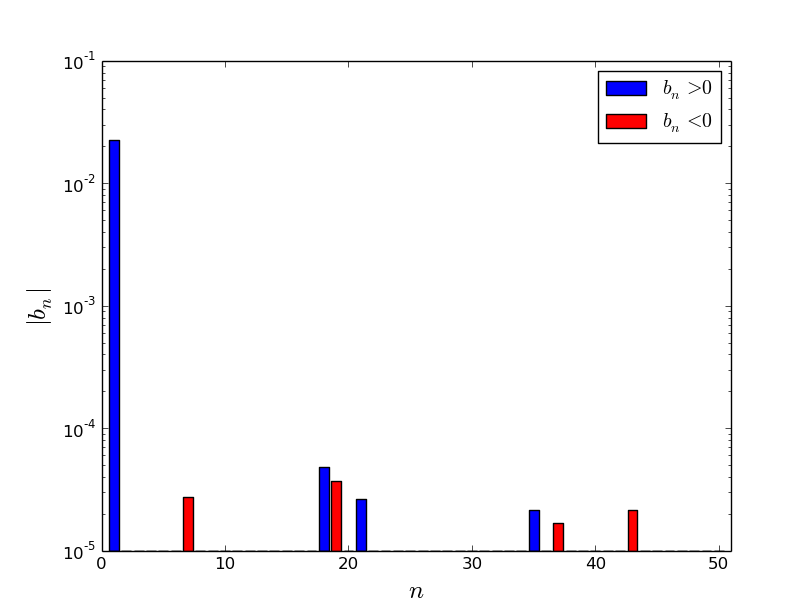
\includegraphics[width=0.5\linewidth] {10.png}
	\caption{Approximate solution coefficients (\ref{15}).}
	\label{fig:3}
  \end{center}
\end{figure} 

We distinguish two phases of the dynamic process: fast and slow. In the fast phase, the initial condition (\ref{14}) 
is rearranged to the initial condition, which corresponds to (\ref{15}): from the function
$\bm u(\bm x, 0)$ to the function $\bm u_N(\bm x, 0)$. The slow phase is associated with the evolution of the solution according to (\ref{15}).
Within the state change modal technology, the fast phase is not modeled at all.

The beginning and the end of the fast phase are illustrated through the calculational data shown in Fig. \ref{fig:4}. The results were obtained with $N=10$. We can note very small changes in the topology of the initial and reconstructed initial conditions. Let us pay attention to the substantial restructuring of the solution, which is illustrated by large changes in the neutron flux amplitudes for the first and second groups.

\begin{figure}[!h]
  \begin{center}
\begin{minipage}{0.051\linewidth}
\center{1} \\
\end{minipage}
\hfill
\begin{minipage}{0.3\linewidth}
\center{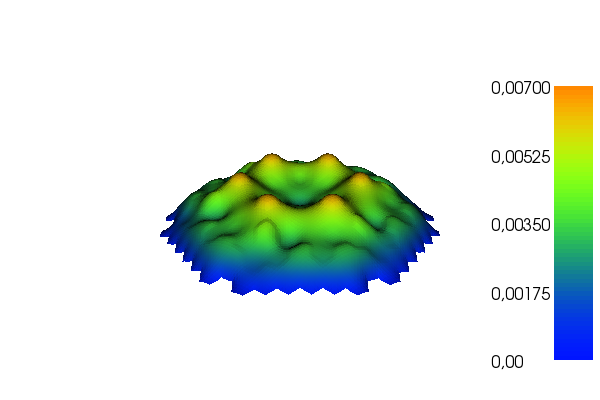
\includegraphics[width=1\linewidth]{11-11.png}} \\
\end{minipage}
\hfill
\begin{minipage}{0.3\linewidth}
\center{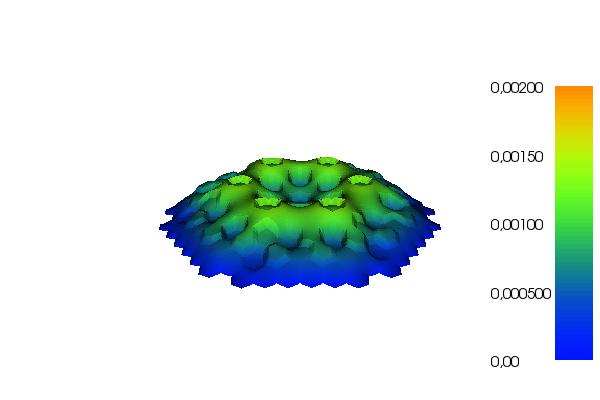
\includegraphics[width=1\linewidth]{11-12.png}} \\
\end{minipage}
\hfill
\begin{minipage}{0.3\linewidth}
\center{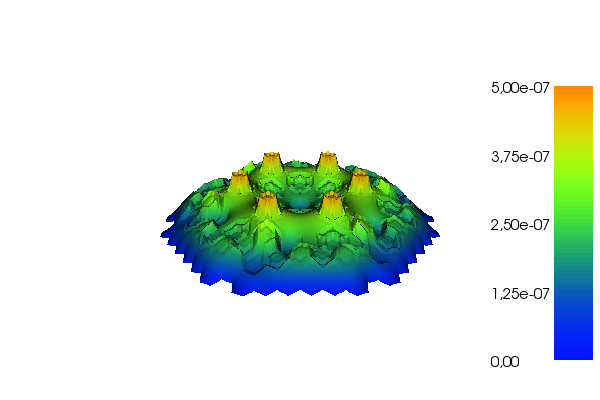
\includegraphics[width=1\linewidth]{11-13.png}} \\
\end{minipage}

\begin{minipage}{0.051\linewidth}
\center{2} \\
\end{minipage}
\hfill
\begin{minipage}{0.3\linewidth}
\center{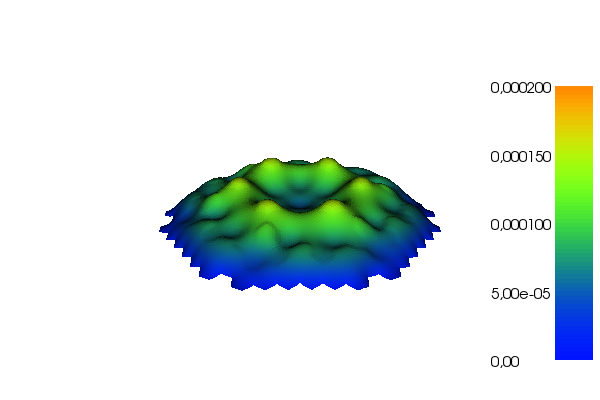
\includegraphics[width=1\linewidth]{11-21.png}} \\
\end{minipage}
\hfill
\begin{minipage}{0.3\linewidth}
\center{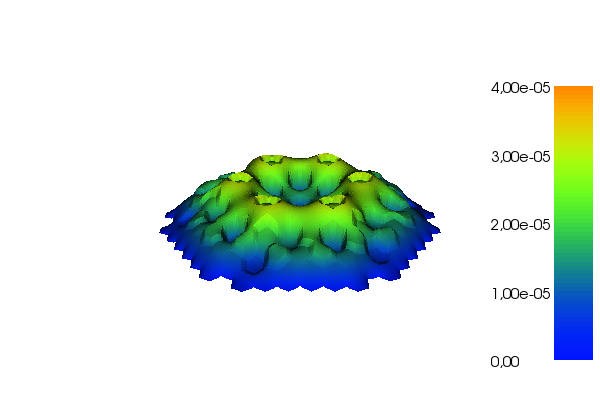
\includegraphics[width=1\linewidth]{11-22.png}} \\
\end{minipage}
\hfill
\begin{minipage}{0.3\linewidth}
\center{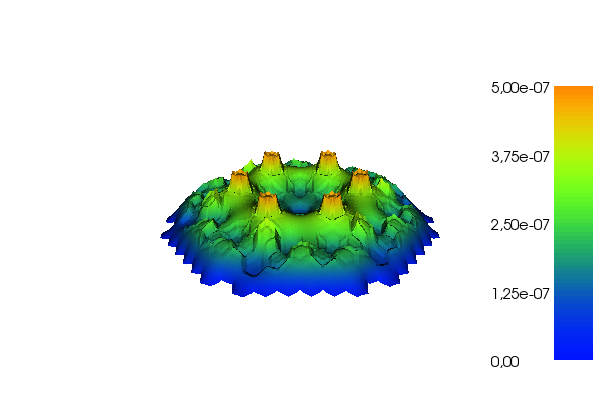
\includegraphics[width=1\linewidth]{11-23.png}} \\
\end{minipage}

\begin{minipage}{0.051\linewidth}
\center{~} \\
\end{minipage}
\hfill
\begin{minipage}{0.3\linewidth}
\center{a} \\
\end{minipage}
\hfill
\begin{minipage}{0.3\linewidth}
\center{b} \\
\end{minipage}
\hfill
\begin{minipage}{0.3\linewidth}
\center{c} \\
\end{minipage}
\hfill

\caption{Function $\bm u(\bm x, 0)$ (string 1) and function  $\bm u_N(\bm x, 0)$ (ctring 2):
a --- neutron flux of group 1, b --- neutron flux of group 2, c --- delayed neutrons source.}
\label{fig:4}
  \end{center}
\end{figure}

\subsection{Comparison with the nonstationary problem solution} 
An approximate solution, obtained using modal approximation, can be compared with the dynamic problem solution (\ref{1}). 
Fully implicit scheme on a uniform grid in time with a sufficiently small step $\tau = 0.0025$ is used (see details in \cite{nd-mm}).
The dynamics of the neutron power of the nuclear reactor $P$ and the delayed neutrons source $C$ at the initial stage during the transition from the critical state to the subcritical in the case of a symmetric perturbation is shown in Fig.\ref{fig:5}. 
Here 
\[
 P(t) = \int_{\Omega} (\nu\Sigma_{f1} \varphi_1 + \nu\Sigma_{f2} \varphi_2)  d \bm x,
 \quad C(t) = \int_{\Omega} c(\bm x,t) d \bm x.
\] 
There is a rapid change in neutron power over a short period of time, while the delayed neutrons sourse changes rather slow. The dynamics of the slow phase is illustrated in Figs. \ref{fig:6}. 
Here the solution of full equations (dynamic in Figs. \ref{fig:6}), and the modal approximation solution (modal) are presented. We see that the integral characteristics of the reactor dynamics at slow stage are calculated with good accuracy.

\begin{figure}[h]
  \begin{center}
    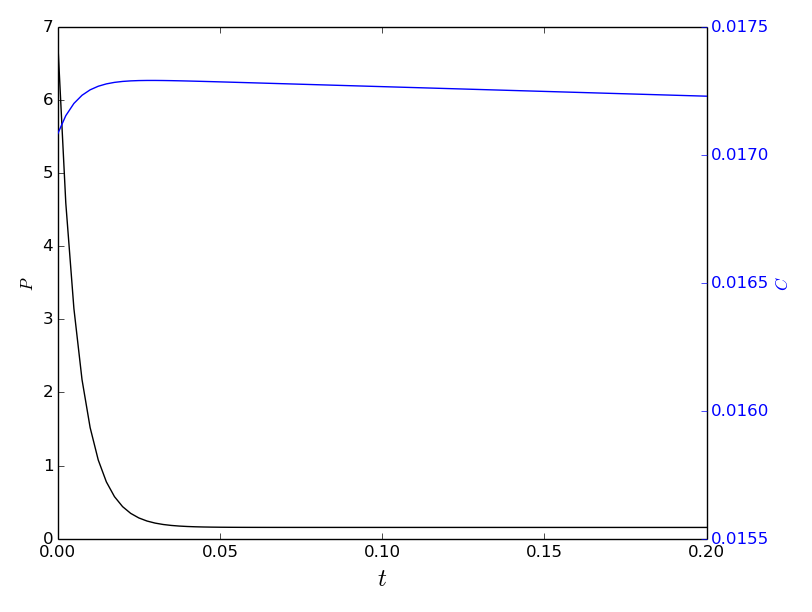
\includegraphics[width=0.5\linewidth] {14.png}
	\caption{Fast stage of reactor state: neutronic power.}
	\label{fig:5}
  \end{center}
\end{figure} 

\begin{figure}[h]
\begin{center}
\begin{minipage}{0.49\linewidth}
    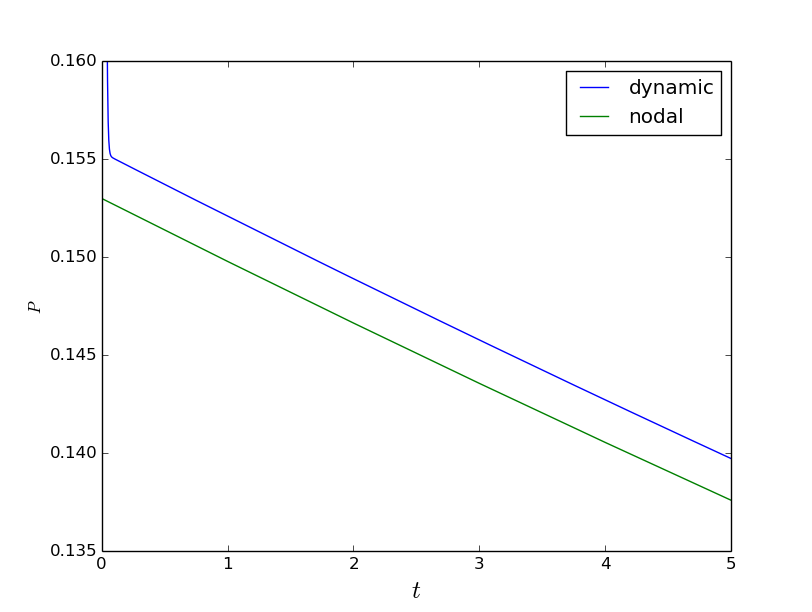
\includegraphics[width=1\linewidth] {15.png}
\end{minipage}
\hfill
\begin{minipage}{0.49\linewidth}
    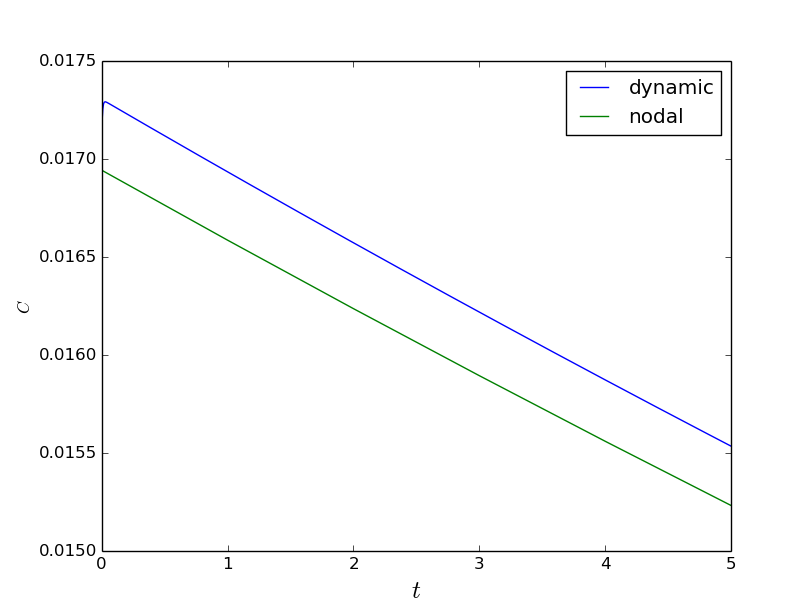
\includegraphics[width=1\linewidth] {16.png}
\end{minipage}
\caption{Slow stage of reactor state: neutronic power and delayed neutrons sourse}
\label{fig:6}
\end{center}
\end{figure}


\clearpage


\section{Conclusions} 

The problem of simulation of reactor dynamic processes is considered on the basis of multigroup neutron diffusion equations accounting for delayed neutrons.
The modal approximation is used: an approximate solution is represented as an expansion on limited number of dominant eigenfunctions of the $\alpha$-eigenvalue spectral problem.

%Numerical simulation of reactor non-stationary processes is carried out on the basis of a successive change in the states of the reactor. These states are characterized by a set of constant parameters to describe the multigroup neutron flux behavior.
%The state change modal method was developed. The phase, which described fast transition to the approximate solution, is selected as a set of dominant modes. At a slow phase of the reactor dynamics, the solution is based on the evolution of dominant modes.
%
%The computational implementation of the state change modal method is based on the previously calculated (of-line calculation) eigenfunctions and eigenvalues of the  $\alpha$-eigenvalue spectral problem. Fast determination of dominant modes and calculation of the reactor neutron flux at selected times are based on on-line calculation.
%The classical Lagrange finite elements $p=1,2,3$ are used for the spatial approximation. 
%Accuracy control is performed using condensed grids. Spectral problems are solved numerically using well-developed free software SLEPc.
%
%Test calculations are made in two-dimensional analysis using a two-group diffusion approximation. Calculations of dominant modes for a reactor supercritical state are performed. The major mode solution, which determines the reactor regular regime, is used as the initial condition for transition to the subcritical state. The modeling of the reactor state change as a transfer from one state to another state is carried out for two cases. The first of them (symmetric perturbation) is due to the uniform change in the absorbing material properties. The second case (asymmetric perturbation) deals with a non-uniform change in the absorbing material properties (in two halves over the reactor cross-section).
%
%Comparison of the calculational results obtained by using two methods (one based on modal approximation and another based on the full dynamics calculation) shows the acceptable accuracy in calculation of neutron power and delayed neutrons source for the VVER-1000 test problem.


\section*{Acknowledgements}
This work are supported by the Russian Foundation for Basic Research (\# 16-08-01215) and by the grant of the Russian Federation Government (\# 14.Y26.31.0013).

\section*{References}
\begin{thebibliography}{50}

\bibitem{iopartnum} IOP Publishing is to grateful Mark A Caprio, Center for Theoretical Physics, Yale University, for permission to include the {\tt iopart-num} \BibTeX package (version 2.0, December 21, 2006) with  this documentation. Updates and new releases of {\tt iopart-num} can be found on \verb"www.ctan.org" (CTAN). 

\bibitem{Ascher2008}
Ascher, U.~M., 2008. Numerical Methods for Evolutionary Differential Equations.
  Society for Industrial Mathematics.

\bibitem{avvakumov2017spectral}
Avvakumov, A.~V., Strizhov, V.~F., Vabishchevich, P.~N., Vasilev, A.~O., 2017.
  Spectral properties of dynamic processes in a nuclear reactor. Annals of
  Nuclear Energy 99, 68--79.

\bibitem{nd-mm}
Avvakumov, A.~V., Vabishchevich, P.~N., Vasilev, A.~O., Strizhov, V.~F., 2016.
  Numerical modelling neutron diffusion unsteady problems. Mathematical Models
  and Computer Simulations~(submitted).

\bibitem{baudron2014parareal}
Baudron, A.-M., Lautard, J.-J., Maday, Y., Riahi, M.~K., Salomon, J., 2014.
  Parareal in time {3D} numerical solver for the {LWR} benchmark neutron
  diffusion transient model. Journal of Computational Physics 279, 67--79.

\bibitem{Bell1970}
Bell, G.~I., Glasstone, S., 1970. Nuclear Reactor Theory. Van Nostrand Reinhold
  Company.

\bibitem{LSPk1996}
Bjõrck, A., 1996. Numerical Methods for Least Squares Problems. Society for
  Industrial and Applied Mathematics.

\bibitem{brenner}
Brenner, S.~C., Scott, R., 2008. The Mathematical Theory of Finite Element
  Methods. Springer.

\bibitem{brezinski1991biorthogonality}
Brezinski, C., 1991. Biorthogonality and Its Applications to Numerical
  Analysis. CRC Press.

\bibitem{Butcher2008}
Butcher, J.~C., 2008. {Numerical Methods for Ordinary Differential Equations}.
  Wiley.

\bibitem{chao}
Chao, Y.~A., Shatilla, Y.~A., 1995. Conformal mapping and hexagonal nodal
  methods-{II}: Implementation in the {ANC-H Code}. Nuclear Science and
  Engineering 121, 210--225.

\bibitem{cho2005fundamentals}
Cho, N.~Z., 2005. Fundamentals and recent developments of reactor physics
  methods. Nuclear Engineering and Technology 37~(1), 25--78.

\bibitem{chou1990three}
Chou, H.~P., Lu, J.~R., Chang, M.~B., 1990. A three-dimensional space-time
  model and its use in pressurized water reactor rod ejection analyses. Nuclear
  Technology 90~(2), 142--154.

\bibitem{dahmani20013d}
Dahmani, M., Baudron, A.~M., Lautard, J.~J., Erradi, L., 2001. A {3D} nodal
  mixed dual method for nuclear reactor kinetics with improved quasistatic
  model and a semi-implicit scheme to solve the precursor equations. Annals of
  Nuclear Energy 28~(8), 805--824.

\bibitem{dodds1976accuracy}
Dodds~Jr, H.~L., 1976. Accuracy of the quasistatic method for two-dimensional
  thermal reactor transients with feedback. Nuclear Science and Engineering
  59~(3), 271--276.

\bibitem{duderstadt1976nuclear}
Duderstadt, J.~J., Hamilton, L.~J., 1976. Nuclear Reactor Analysis. Wiley.

\bibitem{dugan2016cross}
Dugan, K., Zmijarevic, I., Sanchez, R., 2016. Cross-section homogenization for
  reactivity-induced transient calculations. Journal of Computational and
  Theoretical Transport 45~(6), 425--441.

\bibitem{dulla2008quasi}
Dulla, S., Mund, E.~H., Ravetto, P., 2008. The quasi-static method revisited.
  Progress in Nuclear Energy 50~(8), 908--920.

\bibitem{Gear1971}
Gear, C.~W., 1971. {Numerical Initial Value Problems in Ordinary Differential
  Equations}. Prentice Hall, NJ.

\bibitem{ginestar2002transient}
Ginestar, D., Miro, R., Verdu, G., Hennig, D., 2002. A transient modal analysis
  of a {BWR} instability event. Journal of Nuclear Science and Technology
  39~(5), 554--563.

\bibitem{goluoglu2001time}
Goluoglu, S., Dodds, H.~L., 2001. A time-dependent, three-dimensional neutron
  transport methodology. Nuclear science and engineering 139~(3), 248--261.

\bibitem{gonzalez2009high}
Gonz{\'a}lez-Pintor, S., Ginestar, D., Verd{\'u}, G., 2009. High order finite
  element method for the lambda modes problem on hexagonal geometry. Annals of
  Nuclear Energy 36~(9), 1450--1462.

\bibitem{grossman2007nodal}
Grossman, L.~M., Hennart, J.-P., 2007. Nodal diffusion methods for space-time
  neutron kinetics. Progress in Nuclear Energy 49~(3), 181--216.

\bibitem{guerin2010domain}
Gu{\'e}rin, P., Baudron, A.-M., Lautard, J.-J., 2010. Domain decomposition
  methods for the neutron diffusion problem. Mathematics and Computers in
  Simulation 80~(11), 2159--2167.

\bibitem{HairerWanner2010}
Hairer, E., Wanner, G., 2010. {Solving Ordinary Differential Equations II:
  Stiff and Differential-Algebraic Problems}. Springer Verlag.

\bibitem{henry1975nuclear}
Henry, A.~F., 1975. Nuclear-Reactor Analysis. MIT press.

\bibitem{hernandez2005slepc}
Hernandez, V., Roman, J.~E., Vidal, V., 2005. {SLEPc: A} scalable and flexible
  toolkit for the solution of eigenvalue problems. ACM Transactions on
  Mathematical Software (TOMS) 31~(3), 351--362.

\bibitem{hernandez2003resolution}
Hernandez, V., Roman, J.~E., Vidal, V., Verdu, G., Ginestar, D., 2003.
  {Resolution of the neutron diffusion equation with SLEPc, the Scalable
  Library for Eigenvalue Problem Computations}. In: Nuclear Mathematical and
  Computational Sciences: A Century in Review, A Century Anew Gatlinburg.
  American Nuclear Society, pp. 1--10.

\bibitem{hetrick1971dynamics}
Hetrick, D.~L., 1971. Dynamics of Nuclear Reactors. University of Chicago
  Press.

\bibitem{HundsdorferVerwer2003}
Hundsdorfer, W.~H., Verwer, J.~G., 2003. Numerical Solution of Time-Dependent
  Advection-Diffusion-Reaction Equations. Springer Verlag.

\bibitem{Laub2005}
Laub, A.~J., 2005. Matrix Analysis for Scientists and Engineers. Society for
  Industrial and Applied Mathematics.

\bibitem{lawrence1986progress}
Lawrence, R.~D., 1986. Progress in nodal methods for the solution of the
  neutron diffusion and transport equations. Progress in Nuclear Energy 17~(3),
  271--301.

\bibitem{LeVeque2007}
LeVeque, R.~J., 2007. Finite Difference Methods for Ordinary and Partial
  Differential Equations: Steady-State and Time-Dependent Problems. Society for
  Industrial Mathematics.

\bibitem{lewis1993computational}
Lewis, E.~E., Miller, W.~F., 1993. Computational Methods of Neutron Transport.
  American Nuclear Society.

\bibitem{luikov2012analytical}
Luikov, A., 1968. Analytical Heat Diffusion Theory. Academic Press.

\bibitem{maday2005parareal}
Maday, Y., Turinici, G., 2005. The parareal in time iterative solver: a further
  direction to parallel implementation. In: Domain Decomposition Methods in
  Science and Engineering. Springer, pp. 441--448.

\bibitem{marchuk1986numerical}
Marchuk, G.~I., Lebedev, V.~I., 1986. Numerical Methods in the Theory of
  Neutron Transport. Harwood Academic Pub.

\bibitem{miro2002nodal}
Mir{\'o}, R., Ginestar, D., Verd{\'u}, G., Hennig, D., 2002. A nodal modal
  method for the neutron diffusion equation. application to {BWR} instabilities
  analysis. Annals of Nuclear Energy 29~(10), 1171--1194.

\bibitem{modak2007scheme}
Modak, R., Gupta, A., 2007. A scheme for the evaluation of dominant
  time-eigenvalues of a nuclear reactor. Annals of Nuclear Energy 34~(3),
  213--221.

\bibitem{Ortega1987}
Ortega, J.~M., 1987. Matrix Theory: A Second Course. Springer.

\bibitem{quarteroni}
Quarteroni, A., Valli, A., 2008. Numerical Approximation of Partial
  Differential Equations. Springer.

\bibitem{Saad2003}
Saad, Y., 2003. Iterative Methods for Sparse Linear Systems. Society for
  Industrial Mathematics.

\bibitem{Saadbook}
Saad, Y., 2011. Numerical Methods for Large Eigenvalue Problems. SIAM.

\bibitem{Samarskiibook}
Samarskii, A.~A., 2001. The Theory of Difference Schemes. Marcel Dekker, New
  York.

\bibitem{samarskii1996computational}
Samarskii, A.~A., Vabishchevich, P.~N., 1996. Computational Heat Transfer.
  Wiley.

\bibitem{sanchez2009assembly}
Sanchez, R., 2009. Assembly homogenization techniques for core calculations.
  Progress in Nuclear Energy 51~(1), 14--31.

\bibitem{smith1979analytic}
Smith, K.~S., 1979. An analytic nodal method for solving the two-group,
  multidimensional, static and transient neutron diffusion equations. Ph.D.
  thesis, Massachusetts Institute of Technology.

\bibitem{stacey1967modal}
Stacey, W.~M., 1967. Modal Approximations: Theory and an Application to Reactor
  Physics. The MIT Press.

\bibitem{stacey1969space}
Stacey, W.~M., 1969. Space-Time Nuclear Reactor Kinetics. Academic Press.

\bibitem{stacey}
Stacey, W.~M., 2007. Nuclear Reactor Physics. Wiley.

\bibitem{stewart2002krylov}
Stewart, G.~W., 2001. A {Krylov--Schur} algorithm for large eigenproblems. SIAM
  Journal on Matrix Analysis and Applications 23~(3), 601--614.

\bibitem{stewart1976spectral}
Stewart, H.~B., 1976. Spectral theory of heterogeneous diffusion systems.
  Journal of Mathematical Analysis and Applications 54~(1), 59--78.

\bibitem{sutton1996diffusion}
Sutton, T.~M., Aviles, B.~N., 1996. Diffusion theory methods for spatial
  kinetics calculations. Progress in Nuclear Energy 30~(2), 119--182.

\bibitem{ToselliWidlund2005}
Toselli, A., Widlund, O., 2005. Domain Decomposition Methods -- Algorithms and
  Theory. Springer.

\bibitem{VabishchevichSM}
Vabishchevich, P.~N., 2012. {SM}-stability of operator-difference schemes.
  Computational Mathematics and Mathematical Physics 52~(6), 887--894.

\bibitem{Vabishchevich2014}
Vabishchevich, P.~N., 2014. {Additive Operator-Difference Schemes: Splitting
  Schemes}. de Gruyter.

\bibitem{verdu2014modal}
Verd{\'u}, G., Ginestar, D., 2014. Modal decomposition method for {BWR}
  stability analysis using {A}lpha-modes. Annals of Nuclear Energy 67, 31--40.

\bibitem{verdu20103d}
Verdu, G., Ginestar, D., Roman, J., Vidal, V., 2010. {3D} alpha modes of a
  nuclear power reactor. Journal of Nuclear Science and Technology 47~(5),
  501--514.

\bibitem{verdu1998modal}
Verd{\'u}, G., Ginestar, D., Vidal, V., Mir{\'o}, R., 1998. Modal decomposition
  method for {BWR} stability analysis. Journal of Nuclear Science and
  Technology 35~(8), 538--546.

\bibitem{vidal2014solution}
Vidal-Ferrandiz, A., Fayez, R., Ginestar, D., Verd{\'u}, G., 2014. Solution of
  the lambda modes problem of a nuclear power reactor using an h--p finite
  element method. Annals of Nuclear Energy 72, 338--349.
  
\end{thebibliography}

\end{document}


